\section{Bascule}
Un registre est un élément fondamental de l'électronique digitale. Il est utilisé par example dans le processeur de votre téléphone, de votre ordinateur ou encore de votre carte de banque. Ce composant implémente la table de vérité présentée à la Figure~\ref{fig:reg_tab}. Elle permet de visualiser l'effet des entrées (i.e. partie de gauche) sur les sorties (i.e. partie de droite). Par example, on y voit que si le signal \texttt{CLK} est stable ($0$ ou $1$ est noté $x$), alors la sortie ne change pas. Le $Q_{next}$ suivant est le même que $Q$. Elle est donc retenue dans le registre. Celui-ci sert donc de \textbf{mémoire}. Par contre, si le \texttt{CLK} passe de $0$ à $1$, alors l'entrée $D$ passe à la sortie $Q$ et $\bar{Q}$ qui est la négation de $Q$. Ce qui permet de changer la valeur de $Q$ et donc de mémoriser $D$ pour plus tard. 

\begin{table}[h!]
\centering
\begin{tabular}{|c|c || c |c | }
\hline 
\texttt{CLK} & $D$ & $Q_{next}$ & $\bar{Q}_{next}$\\ \hline \hline
x   & x   & $Q$   & $\bar{Q}$ \\ \hline
$0\to1$ & $0$ & $0$ & $1$ \\ \hline 
$0\to1$ & $1$ & $1$ & $0$ \\ \hline 
\end{tabular}
    \caption{Table de vérité d'un registre, (Latch signifie que rien ne change)}
    \label{fig:reg_tab}
\end{table}

Afin de reproduire le comportement de la Figure~\ref{fig:signal-all_HO3}, un registre peut être connecté comme montré à la Figure~\ref{fig:DFFbascule}. Là, l'entrée $D$ est fixée à $\bar{Q}$ qui est la négation de la sortie ($\bar{Q}$). Ainsi, une fois que \texttt{CLK} passera de $0$ à $1$, le signal de sortie sera inversé. Faites correspondre pas à pas la Figure~\ref{fig:signal-all_HO3} ainsi que la table de vérité pour bien comprendre le fonctionnement du circuit. Bien que le port du \texttt{CD4013BE} soit appelé \texttt{CLK}, nous utilisons le signal provenant du HO2 pour contrôler la bascule. C'est donc le signal carré (flan montant) de la Figure \ref{fig:signal-all} qui gère le changement d'état du registre. \\

\begin{figure}[h!]
    \centering
    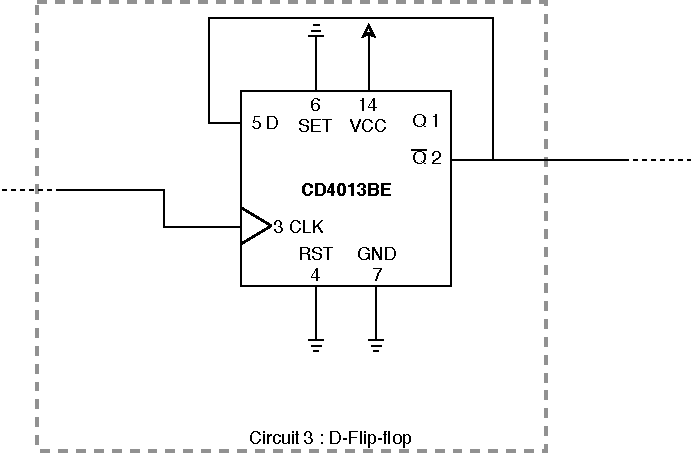
\includegraphics[width=0.6\textwidth]{HO3_dff.pdf}
    \caption{Registre en mode bascule}
    \label{fig:DFFbascule}
\end{figure}
\medskip

